\documentclass{article}

% if you need to pass options to natbib, use, e.g.:
% \PassOptionsToPackage{numbers, compress}{natbib}
% before loading nips_2017
%
% to avoid loading the natbib package, add option nonatbib:
% \usepackage[nonatbib]{nips_2017}

%\usepackage{main}

% to compile a camera-ready version, add the [final] option, e.g.:
\usepackage[final]{main}

\usepackage[utf8]{inputenc} % allow utf-8 input
\usepackage[T1]{fontenc}    % use 8-bit T1 fonts
\usepackage{hyperref}       % hyperlinks
\usepackage{url}            % simple URL typesetting
\usepackage{booktabs}       % professional-quality tables
\usepackage{amsfonts}       % blackboard math symbols
\usepackage{nicefrac}       % compact symbols for 1/2, etc.
\usepackage{microtype}      % microtypography
\usepackage{multicol}
\usepackage{graphicx}
\usepackage{amsmath}
\usepackage{bm}
\usepackage{bbm}
\usepackage{enumerate}
\usepackage[linguistics]{forest}
\usepackage{adjustbox}
\usepackage{amssymb}
\usepackage{mathtools}
\DeclarePairedDelimiter{\ceil}{\lceil}{\rceil}
\DeclarePairedDelimiter{\floor}{\lfoor}{\rfloor}
%\usepackage[margin=0.5in]{geometry}
%\DeclareMathOperator*{\argmax}{argmax}

\usepackage{listings}
\usepackage{color}
\usepackage{longtable}

\usepackage{tikz}
\usetikzlibrary{shapes.geometric, arrows}
\tikzstyle{startstop} = [rectangle, rounded corners, minimum width=3cm, minimum height=1cm,text centered, draw=black, fill=red!30]
\tikzstyle{io} = [trapezium, trapezium left angle=70, trapezium right angle=110, minimum width=3cm, minimum height=1cm, text centered, draw=black, fill=blue!30]
% \tikzstyle{process} = [rectangle, minimum width=3cm, minimum height=1cm, text centered, draw=black, fill=orange!30]
\tikzstyle{process} = [rectangle, minimum width=3cm, minimum height=1cm, text centered, text width=3cm, draw=black, fill=orange!30]
\tikzstyle{decision} = [diamond,  minimum width=3cm, aspect=2, text centered, text width=3cm, draw=black, fill=green!30]
\tikzstyle{arrow} = [thick,->,>=stealth]

\usepackage{fancyhdr}
\pagestyle{fancy}
\fancyhf{}
\renewcommand{\headrulewidth}{0pt}
\lfoot{\href{https://www.overleaf.com/read/jjqbcnmkcgcg}{\underline{Link}} to the Overleaf Project.}
\rfoot{\thepage}

\newcommand{\matr}[1]{\bm{#1}}     % ISO complying version
\newcommand{\vect}[1]{\bm{#1}}     % ISO complying version
 
\definecolor{codegreen}{rgb}{0,0.6,0}
\definecolor{codegray}{rgb}{0.5,0.5,0.5}
\definecolor{codepurple}{rgb}{0.58,0,0.82}
\definecolor{backcolour}{rgb}{0.95,0.95,0.92}
 
\lstdefinestyle{mystyle}{
    backgroundcolor=\color{backcolour},   
    commentstyle=\color{codegreen},
    keywordstyle=\color{magenta},
    numberstyle=\ttfamily\tiny\color{codegray},
    stringstyle=\color{codepurple},
    basicstyle=\ttfamily\small,
    columns=fullflexible,
    breakatwhitespace=false,         
    breaklines=true,                 
    captionpos=t,                    
    keepspaces=true,                 
    numbers=left,                    
    numbersep=5pt,                  
    showspaces=false,                
    showstringspaces=false,
    showtabs=false,                  
    tabsize=4,
}

\hypersetup{colorlinks=true}
 
\lstset{style=mystyle}

\title{Deep Learning - Spring 2019\\
       \Large Homework 3}
\graphicspath{{images/}}
\setcitestyle{round, sort, numbers}

% The \author macro works with any number of authors. There are two
% commands used to separate the names and addresses of multiple
% authors: \And and \AND.
%
% Using \And between authors leaves it to LaTeX to determine where to
% break the lines. Using \AND forces a line break at that point. So,
% if LaTeX puts 3 of 4 authors names on the first line, and the last
% on the second line, try using \AND instead of \And before the third
% author name.

\author{
  Daniel Rivera Ruiz\\
  Department of Computer Science\\
  New York University\\
  \href{mailto:drr342@nyu.edu}{\texttt{drr342@nyu.edu}}\\
}

\begin{document}

\maketitle

% \cite{} - in-line citation author, year in parenthesis.
% \citep{} - all citation info in parenthesis.

%	\begin{figure}[ht]
%		\centering
%		\frame{
%            \includegraphics[width=1.0\linewidth]{tree.png}
%       }
%		\caption{Classification results for the sentence \textit{"There are slow and repetitive parts, but it has just enough spice to keep it                  interesting."} using the Stanford Sentiment Treebank. As can be seen, sentiment scores are available for each phrase.}
%		\label{tree}
%	\end{figure}

\section{Fundamentals}
\subsection{Dropout}
Dropout is a very popular regularization technique.
\begin{itemize}
    \item[(a)] List the \texttt{torch.nn} module corresponding to 2D dropout.
    
    \texttt{torch.nn.Dropout2d(p=0.5, inplace=False)}. Randomly zero out entire channels of the input tensor. Each channel will be zeroed out independently on every forward call with probability $p$ using samples from a Bernoulli distribution.
    
    \item[(b)] Read on what dropout is and give a short explanation on what it does and why it is useful.
    
    Dropout provides a method of regularizing a broad family of models. To a first approximation, it makes bagging practical for ensembles of very large neural networks. More specifically, dropout trains the ensemble consisting of all sub-networks that can be formed by removing non-output units from an underlying base network. In most modern neural networks, we can achieve this by multiplying its output value by zero.
    
    One advantage of dropout is that it is computationally cheap: using dropout during training requires only $O(n)$ computations per example per update. Another significant advantage is that it does not limit the type of model or training procedure that can be used: it works well with nearly any model that uses a distributed representation and can be trained with stochastic gradient descent.
    
    Though the cost per step of applying dropout to a specific model is negligible, the cost of using it in a complete system can be significant. Typically, the optimal validation set error is much lower when using dropout, but this comes at the cost of a much larger model and many more iterations of the training algorithm. 

    It is worth noticing that dropout trains an ensemble of models that share hidden units. This means each hidden unit must be able to perform well regardless of which other hidden units are in the model. Dropout thus regularizes each hidden unit to be not merely a good feature but a feature that is good in many contexts.
\end{itemize}

\newpage

\subsection{Batch Normalization}
\begin{itemize}
    \item[(a)] What does mini-batch refer to in the context of deep learning?
    
    In the context of deep learning, mini-batch refers to a partition of the training dataset that is used to calculate a model's error and update its coefficients. Mini-batch gradient descent is a variation of the gradient descent algorithm that uses mini-batches and is the most common implementation of gradient descent in the field of deep learning. Mini-batch gradient descent seeks to find a balance between the robustness of stochastic gradient descent and the efficiency of batch gradient descent.
    
    \item[(b)] Read on what batch normalization is and give a short explanation on what it does and why it is useful.
    
    Batch normalization is a method of adaptive reparametrization motivated by the difficulty of training very deep neural networks. In these models, the gradient tells how to update each parameter assuming that the other layers do not change. In practice, however, unexpected results can arise because many functions composed together are changed simultaneously, using updates that were computed under the assumption that the other functions remain constant.
    
    Batch normalization provides an elegant way of reparametrizing almost any deep network that reduces the problem of coordinating updates across many layers. Let $\matr{H}$ be a mini-batch of activations of the layer to normalize arranged as a design matrix. To normalize $\matr{H}$, we replace it with 
    \begin{equation*}
        \hat{\matr{H}} = \frac{\matr{H}-\vect{\mu}}{\vect{\sigma}}
    \end{equation*}
    where $\vect{\mu}$ is a vector containing the mean of each unit and $\vect{\sigma}$ is a vector containing the standard deviation of each unit.
    
    The normalization of a unit can reduce the expressive power of the neural network that contains it. To avoid this, it is common to replace the batch of hidden unit activations $\matr{H}$ with $\gamma\hat{\matr{H}}+\beta$ rather than simply the normalized $\hat{\matr{H}}$. The variables $\gamma$ and $\beta$ are learned parameters that allow the new variable to have any mean and standard deviation. This new parametrization can represent the same family of functions as the old parametrization, but with different learning dynamics. Instead of depending on complicated interactions between the parameters in the layers below, the mean of the new parametrization is determined solely by $\beta$, which makes it much easier to learn with gradient descent.
\end{itemize}

\newpage

\section{Language Modeling}
This exercise explores the code from the \href{https://github.com/pytorch/examples/blob/master/word_language_model}{\texttt{word\_language\_model}} example in \emph{PyTorch}.
\begin{itemize}
    \item[(a)] Go through the code and draw a block diagram / flow chart which highlights the main interacting components, illustrates their functionality, and provides an estimate of their computational time percentage (rough profiling).
    
	\begin{figure}[ht]
	\centering
    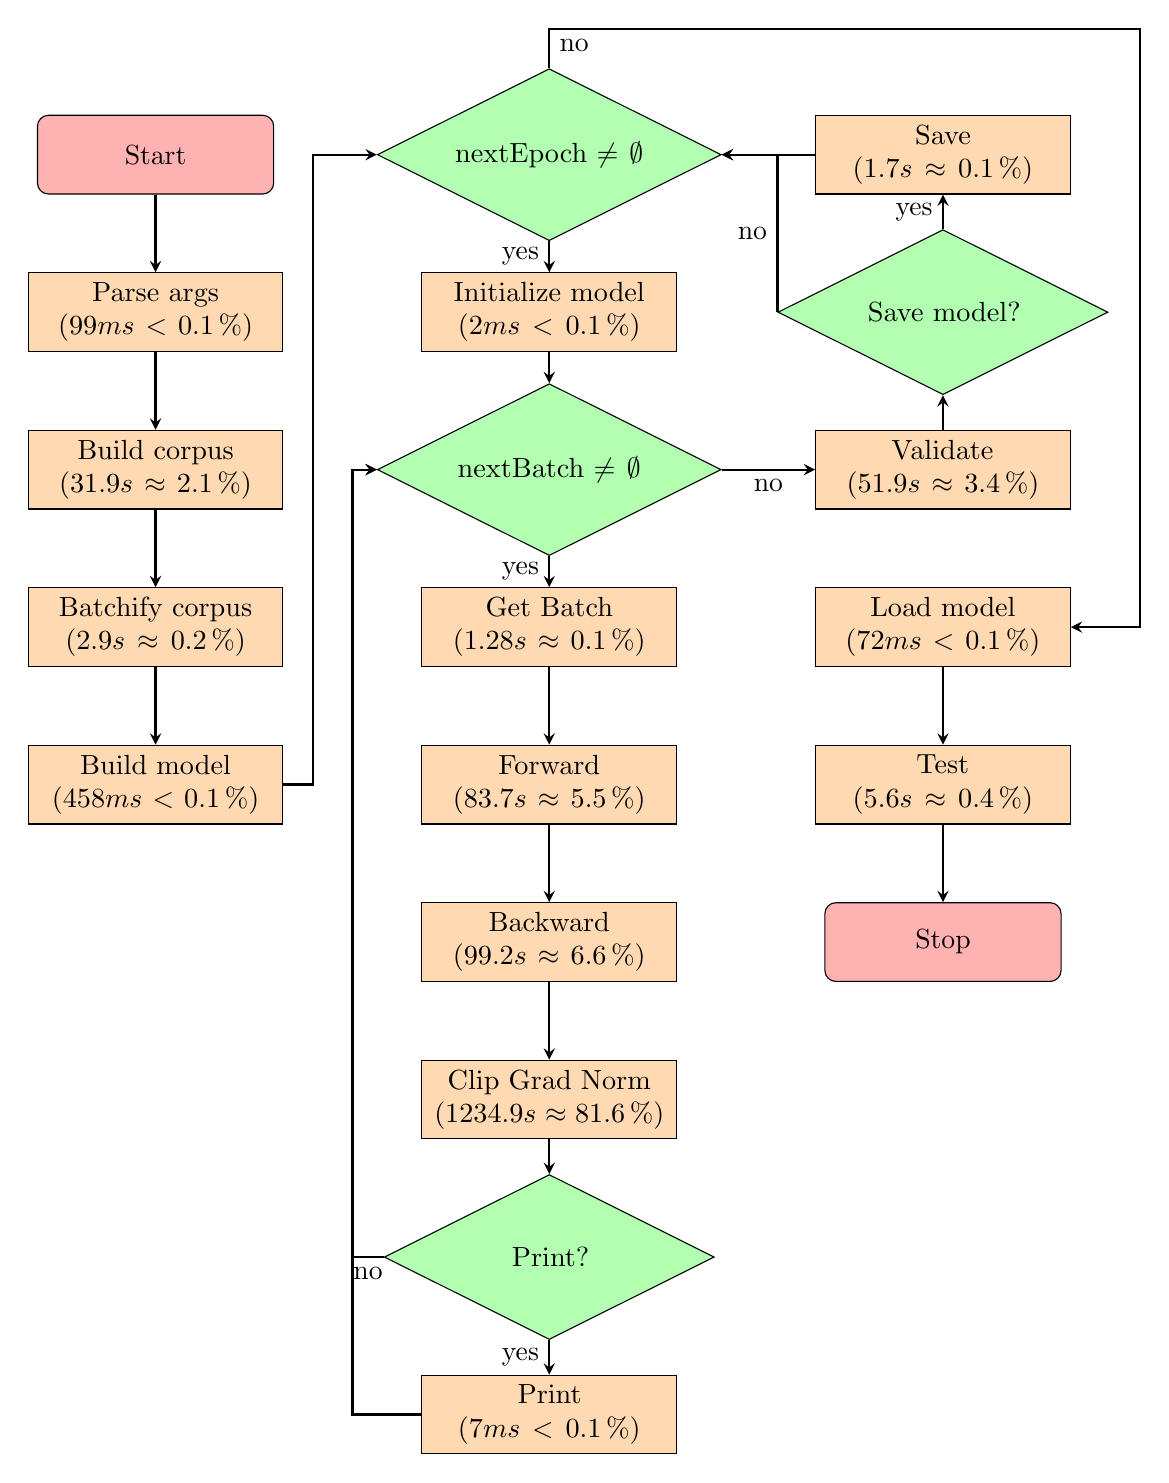
\begin{tikzpicture}[node distance=2cm]
        \node (start) [startstop] {Start};
        \node (parse) [process, below of=start] {Parse args\\ $(99ms < 0.1\,\%)$};
        \node (corpus) [process, below of=parse] {Build corpus\\ $(31.9s \approx 2.1\,\%)$};
        \node (batchify) [process, below of=corpus] {Batchify corpus\\ $(2.9s  \approx 0.2\,\%)$};
        \node (model) [process, below of=batchify] {Build model\\ $(458ms < 0.1\,\%)$};
        \node (forLoop) [decision, right of=start, xshift=3cm] {nextEpoch $\neq \emptyset$};
        \node (init) [process, below of=forLoop] {Initialize model\\ $(2ms < 0.1\,\%)$};
        \node (nextBatch) [decision, below of=init] {nextBatch $\neq \emptyset$};
        \node (getBatch) [process, below of=nextBatch] {Get Batch\\ $(1.28s \approx 0.1\,\%)$};
        \node (forward) [process, below of=getBatch] {Forward\\ $(83.7s \approx 5.5\,\%)$};
        \node (backward) [process, below of=forward] {Backward\\ $(99.2s \approx 6.6\,\%)$};
        \node (clip) [process, below of=backward] {Clip Grad Norm\\ $(1234.9s \approx 81.6\,\%)$};
        \node (print?) [decision, below of=clip] {Print?};
        \node (print) [process, below of=print?] {Print\\ $(7ms < 0.1\,\%)$};
        \node (eval) [process, right of=nextBatch, xshift=3cm] {Validate\\ $(51.9s \approx 3.4\,\%)$};
        \node (save?) [decision, above of=eval] {Save model?};
        \node (save) [process, above of=save?] {Save\\ $(1.7s \approx 0.1\,\%)$};
        \node (load) [process, below of=eval] {Load model\\ $(72ms < 0.1\,\%)$};
        \node (test) [process, below of=load] {Test\\ $(5.6s \approx 0.4\,\%)$};
        \node (stop) [startstop, below of=test] {Stop};
        
        \draw [arrow] (start) -- (parse);
        \draw [arrow] (parse) -- (corpus);
        \draw [arrow] (corpus) -- (batchify);
        \draw [arrow] (batchify) -- (model);
        \draw [arrow] (model) -- +(2,0) |- (forLoop.west);
        \draw [arrow] (forLoop) -- node[anchor=east] {yes} (init);
        \draw [arrow] (init) -- (nextBatch);
        \draw [arrow] (nextBatch) -- node[anchor=east] {yes} (getBatch);
        \draw [arrow] (getBatch) -- (forward);
        \draw [arrow] (forward) -- (backward);
        \draw [arrow] (backward) -- (clip);
        \draw [arrow] (clip) -- (print?);
        \draw [arrow] (print?) -- node[anchor=east] {yes} (print);
        \draw [arrow] (print?) -- node[anchor=north] {no} +(-2.5,0) |- (nextBatch.west);
        \draw [arrow] (print) -- +(-2.5,0) |- (nextBatch.west);
        \draw [arrow] (nextBatch) -- node[anchor=north] {no} (eval);
        \draw [arrow] (eval) -- (save?);
        \draw [arrow] (save?) -- node[anchor=east] {yes} (save);
        \draw [arrow] (save) -- (forLoop);
        \draw [arrow] (save?.west) -- node[anchor=east] {no} +(0,2) -- (forLoop);
        \draw [arrow] (forLoop.north) |- node[anchor=north west] {no} +(7.5,0.5) |- (load.east);
        \draw [arrow] (load) -- (test);
        \draw [arrow] (test) -- (stop);
    \end{tikzpicture}
	\caption{Flow diagram for the \texttt{word\_language\_model} application. The percentage execution times were calculated by running \texttt{main.py} on a Tesla K80 GPU for 10 epochs and all other parameters set to default values.}
	\label{fig1}
	\end{figure}
	
	In addition to  the time percentages shown in the flow chart, which were generated by manually adding \texttt{time.time()} commands through out the code, figure \ref{fig2} shows the profiling results obtained with \texttt{cProfile}. In both cases we can see that most of the running time is spent in clipping the gradient and updating the parameters of the model, followed by the backward and forward passes of the training stage.
	
	\begin{figure}[ht]
		\centering
        \includegraphics[width=1.0\linewidth]{cProfile.PNG}
		\caption{Profiling results using the \texttt{cProfile} command (Top 10 results sorted by time are shown).}
		\label{fig2}
	\end{figure}
    
    \item[(b)] Find and explain where and how the back-propagation through time (BPTT) takes place (you may need to delve into \emph{PyTorch} source code).\\
    In the original source code, \href{https://github.com/pytorch/examples/blob/master/word_language_model/main.py#L155-L159}{these lines} are the ones responsible for the forward and backward propagation of the model. In particular, BPTT (as well as regular back-propagation) takes place when we call \texttt{loss.backward()}. This function calculates the gradient of the loss with respect to all the relevant variables in the computational graph and updates the \texttt{.grad} field for all of them. What makes BPTT different (which is explained in detail in the next question) is that we do not back-propagate the dependencies of the hidden states until time zero, but only for a fixed number of time steps. This will limit the scope of the model's memory but will mitigate the effects of vanishing or exploding gradients.\\
    The way this works is by means of the \texttt{detach()} function, which is at the core of \texttt{repackage\_hidden()}. When we detach the hidden state tensor before the forward pass of the model, we are effectively setting its \texttt{grad\_fn} attribute to \texttt{None} (The definition of \texttt{detach()} in \emph{PyTorch} source code can be found \href{https://github.com/pytorch/pytorch/blob/master/torch/tensor.py#L176-L179}{here}, but the actual implementation is written in C++. The attribute \texttt{grad\_fn} is a reference to the computational graph that was used to calculate the tensor. Therefore, when we set it to \texttt{None} the tensor forgets its history (how it was created) and gradient can no longer be backpropagated through it (this can be seen in the \emph{PyTorch} source code \href{https://github.com/pytorch/pytorch/blob/master/torch/nn/modules/module.py#L505-L510}{here}).  
    \item[(c)] Describe why we need the \texttt{repackage\_hidden(h)} function, and how it works.\\
    As it is briefly explained in the code comments, at the beginning of each batch is necessary to detach the hidden state from the computational graph that produced it, i.e. generate a copy of the tensor that does not have any references as to how it was generated and therefore gradient cannot be backpropagated through it. If we don't do this, the model would try to backpropagate through time all the way to the beginning of the dataset.\\
    The way \texttt{repackage\_hidden(h)} works is quite simple: if \texttt{h} is a tensor, it returns \texttt{h.detach()}. Otherwise, it returns a tuple containing all the detached versions of the elements in \texttt{h} (so for the function to work \texttt{h} must be either a tensor or a collection of tensors).\\
    \item[(d)] Why is there a \texttt{---tied (tie the word embedding and softmax weights)} option?\\
    This option is used to tie together the weights associated to the encoder module (word embeddings) and the weights associated to the decoder module (hidden linear layer). "Tying together" basically means that both modules will share the same weights. In order to use this option, the dimension of the word embeddings \texttt{(---emsize)} and the number of hidden units in the linear layer \texttt{(---nhid)} must coincide. For higher dimensions, tying these weights reduces considerably the size of the model (making it faster to train and evaluate) while yielding similar results.\\
    \item[(e)] Compare LSTM and GRU performance (validation perplexity and training time) for different values of the following parameters: number of epochs, number of layers, hidden units size, input embedding dimensionality, BPTT temporal interval, and non-linearities (pick just 3 of these parameters and experiment with 2-3 different values for each).\\
    Table \ref{tb1} shows the results (accumulated training time, final validation perplexity and best validation perplexity) of 27 experiments for each model type. The modified parameters in each experiment were input embedding dimensionality, number of layers and BPTT temporal interval. The models were trained for 10 epochs and all other parameters were set to the default values. To obtain comparable results, all the experiments were run on Tesla K80 GPUs available on NYU's Prince HPC Cluster.\\
    
	\begin{longtable}{cccccr}
	    \caption{Models Comparison} \label{tb1} \\
		\toprule
         & & & & Training & Validation \\
		Model & \texttt{emsize} & \texttt{nlayers} & \texttt{bptt} & Time $(s)$ & Perplexity \\
		\midrule
		\endfirsthead
		\toprule
		 & & & & Training & Validation \\
		Model & \texttt{emsize} & \texttt{nlayers} & \texttt{bptt} & Time $(s)$ & Perplexity \\
		\midrule
		\endhead
        LSTM & 100 & 1 & 16 & 1\,450 & 141.40 \\
        LSTM & 100 & 1 & 32 & 1\,240 & 131.63 \\
        LSTM & 100 & 1 & 64 & \textbf{1\,090} & 146.32 \\
        LSTM & 100 & 2 & 16 & 1\,730 & 138.73 \\
        LSTM & 100 & 2 & 32 & 1\,580 & 154.84 \\
        LSTM & 100 & 2 & 64 & 1\,240 & 140.03 \\
        LSTM & 100 & 4 & 16 & 2\,540 & 147.11 \\
        LSTM & 100 & 4 & 32 & 2\,150 & 159.18 \\
        LSTM & 100 & 4 & 64 & 1\,970 & \textbf{166.24} \\
        \midrule
        LSTM & 200 & 1 & 16 & 1\,490 & 140.48 \\
        LSTM & 200 & 1 & 32 & 1\,210 & 130.17 \\
        LSTM & 200 & 1 & 64 & 1\,140 & 141.92 \\
        LSTM & 200 & 2 & 16 & 1\,820 & 158.80 \\
        LSTM & 200 & 2 & 32 & 1\,490 & \textbf{127.78} \\
        LSTM & 200 & 2 & 64 & 1\,220 & 140.41 \\
        LSTM & 200 & 4 & 16 & 2\,580 & 134.58 \\
        LSTM & 200 & 4 & 32 & 2\,140 & 164.88 \\
        LSTM & 200 & 4 & 64 & 2\,150 & 161.78 \\
        \midrule
        LSTM & 400 & 1 & 16 & 1\,630 & 142.58 \\
        LSTM & 400 & 1 & 32 & 1\,380 & 133.41 \\
        LSTM & 400 & 1 & 64 & 1\,160 & 141.07 \\
        LSTM & 400 & 2 & 16 & 1\,930 & 134.58 \\
        LSTM & 400 & 2 & 32 & 1\,580 & 140.64 \\
        LSTM & 400 & 2 & 64 & 1\,360 & 137.95 \\
        LSTM & 400 & 4 & 16 & \textbf{2\,720} & 150.73 \\
        LSTM & 400 & 4 & 32 & 2\,250 & 138.40 \\
        LSTM & 400 & 4 & 64 & 2\,100 & 155.09 \\
        \midrule
        \midrule
        GRU & 100 & 1 & 16 & 1\,390 & 216.92 \\
        GRU & 100 & 1 & 32 & 1\,170 & 142.91 \\
        GRU & 100 & 1 & 64 & \textbf{1\,080} & 134.84 \\
        GRU & 100 & 2 & 16 & 1\,660 & 256.56 \\
        GRU & 100 & 2 & 32 & 1\,440 & 249.34 \\
        GRU & 100 & 2 & 64 & 1\,210 & 133.33 \\
        GRU & 100 & 4 & 16 & 2\,400 & 1\,052.29 \\
        GRU & 100 & 4 & 32 & 2\,090 & 1\,013.71 \\
        GRU & 100 & 4 & 64 & 1\,840 & 982.62 \\
        \midrule
        GRU & 200 & 1 & 16 & 1\,550 & 183.94 \\
        GRU & 200 & 1 & 32 & 1\,330 & 133.61 \\
        GRU & 200 & 1 & 64 & 1\,090 & 135.74 \\
        GRU & 200 & 2 & 16 & 1\,760 & 218.30 \\
        GRU & 200 & 2 & 32 & 1\,510 & 253.57 \\
        GRU & 200 & 2 & 64 & 1\,260 & 132.14 \\
        GRU & 200 & 4 & 16 & 2\,480 & 347.48 \\
        GRU & 200 & 4 & 32 & 2\,070 & 1\,035.86 \\
        GRU & 200 & 4 & 64 & 1\,840 & 1\,040.37 \\
        \midrule
        GRU & 400 & 1 & 16 & 1\,610 & 169.88 \\
        GRU & 400 & 1 & 32 & 1\,290 & 134.28 \\
        GRU & 400 & 1 & 64 & 1\,150 & 137.01 \\
        GRU & 400 & 2 & 16 & 1\,880 & 230.05 \\
        GRU & 400 & 2 & 32 & 1\,490 & 138.71 \\
        GRU & 400 & 2 & 64 & 1\,310 & \textbf{131.29} \\
        GRU & 400 & 4 & 16 & \textbf{2\,530} & 1\,024.61 \\
        GRU & 400 & 4 & 32 & 2\,160 & \textbf{1\,088.03} \\
        GRU & 400 & 4 & 64 & 1\,870 & 977.15 \\
		\bottomrule
	\end{longtable}
    
    \item[(f)] Why do we compute performance on a test set as well? What is this number good for?\\
    The performance metrics (loss and perplexity) measured on the test set are the ones that must be reported as the results of our model because they are the truthful indicators of how good the model generalizes (learns). The metrics obtained on the training and validation sets are not good for this because they are based on data that was used to learn parameters and tune hyperparameters (e.g. learning rate) and therefore tend to be positively biased. The test set performance metrics can be used, for example, to compare two or more methods.
\end{itemize}

\end{document}